\documentclass[11pt]{article}
\usepackage{amsmath, amssymb, physics, mathtools, bm}
\usepackage{tikz, pgfplots}
\pgfplotsset{compat=1.18}
\usepackage[margin=2.3cm]{geometry}
\usepackage{siunitx, booktabs, hyperref}
\usepackage{braket}

\newcommand{\D}{\mathrm{D}}
\newcommand{\de}{\mathrm{d}}
\newcommand{\pd}[2]{\frac{\partial #1}{\partial #2}}
\newcommand{\pdd}[2]{\frac{\partial^{2} #1}{\partial #2^{2}}}
\newcommand{\Lap}{\nabla^{2}}

\title{B5 General Relativity --- Model Solutions, Trinity 2022}
\author{}
\date{}

\begin{document}
\maketitle

%==============================================================
\section*{Question 1 --- Riemann tensor, Bianchi identity, Newtonian limit}

\textbf{Problem.} State Riemann symmetries; interpret the Bianchi identity and contract it to obtain the divergence-free Einstein tensor; recast Einstein's equation as $R_{\mu\nu}=C S_{\mu\nu}$; in the Newtonian (weak, static) limit show $R_{00}=\tfrac12 \Lap g_{00}$ and fix $C$ by matching Poisson's equation.

\subsection*{(a) Symmetries of the Riemann tensor}

With all indices lowered, $R_{\lambda\mu\nu\kappa}$ has:
\begin{align*}
\text{Antisymmetry in first pair:}\quad & R_{\lambda\mu\nu\kappa}=-R_{\mu\lambda\nu\kappa},\\
\text{Antisymmetry in second pair:}\quad & R_{\lambda\mu\nu\kappa}=-R_{\lambda\mu\kappa\nu},\\
\text{Pair-exchange symmetry:}\quad & R_{\lambda\mu\nu\kappa}=R_{\nu\kappa\lambda\mu},\\
\text{First Bianchi (cyclic):}\quad & R_{\lambda\mu\nu\kappa}+R_{\lambda\nu\kappa\mu}+R_{\lambda\kappa\mu\nu}=0.
\end{align*}
Independent components in $D=4$: $20$.

\subsection*{(b) Meaning of ``;'' and contracted Bianchi identity}

\textbf{Notation.} ``$;\eta$'' denotes the covariant derivative $\nabla_\eta$:
\[ T_{\dots;\eta}=\partial_\eta T_{\dots}+\text{(Christoffel terms, one per index)}. \]
It generalises $\partial_\eta$ to curved spacetime, transforming as a tensor.

\textbf{Contracted Bianchi.} Start from
\begin{equation}
R_{\lambda\mu\nu\kappa;\eta}+R_{\lambda\mu\eta\nu;\kappa}+R_{\lambda\mu\kappa\eta;\nu}=0.
\label{eq:bianchi}
\end{equation}
Contract with $g^{\lambda\nu}$ (metric is covariantly constant, $g^{\lambda\nu}{}_{;\alpha}=0$):
\[ g^{\lambda\nu}R_{\lambda\mu\nu\kappa;\eta}+g^{\lambda\nu}R_{\lambda\mu\eta\nu;\kappa}+g^{\lambda\nu}R_{\lambda\mu\kappa\eta;\nu}=0. \]
Use antisymmetry to identify the first contraction: $g^{\lambda\nu}R_{\lambda\mu\nu\kappa}=R^{\nu}{}_{\mu\nu\kappa}=-R^{\nu}{}_{\mu\kappa\nu}=R_{\mu\kappa}$:
\[ R_{\mu\kappa;\eta}+g^{\lambda\nu}R_{\lambda\mu\eta\nu;\kappa}+R^{\nu}{}_{\mu\kappa\eta;\nu}=0. \]
Use the defining contraction $g^{\lambda\nu}R_{\lambda\mu\eta\nu}=R^{\nu}{}_{\mu\eta\nu}=-R_{\mu\eta}$:
\[ R_{\mu\kappa;\eta}-R_{\mu\eta;\kappa}+R^{\nu}{}_{\mu\kappa\eta;\nu}=0. \]
Contract with $g^{\mu\kappa}$:
\[ g^{\mu\kappa}R_{\mu\kappa;\eta}-g^{\mu\kappa}R_{\mu\eta;\kappa}+g^{\mu\kappa}R^{\nu}{}_{\mu\kappa\eta;\nu}=0. \]
Identify $g^{\mu\kappa}R_{\mu\kappa}=R$ in the first term:
\[ R_{;\eta}-g^{\mu\kappa}R_{\mu\eta;\kappa}+g^{\mu\kappa}R^{\nu}{}_{\mu\kappa\eta;\nu}=0. \]
Raise an index in the second term, $g^{\mu\kappa}R_{\mu\eta}=R^{\kappa}{}_{\eta}$:
\[ R_{;\eta}-R^{\kappa}{}_{\eta;\kappa}+g^{\mu\kappa}R^{\nu}{}_{\mu\kappa\eta;\nu}=0. \]
For the last term, use pair-exchange $R_{\lambda\mu\kappa\eta}=R_{\kappa\eta\lambda\mu}$ to get $g^{\mu\kappa}R^{\nu}{}_{\mu\kappa\eta}=-R^{\nu}{}_{\eta}$:
\[ R_{;\eta}-R^{\kappa}{}_{\eta;\kappa}-R^{\nu}{}_{\eta;\nu}=0. \]
Relabel and combine the last two terms:
\[ R_{;\eta}-2R^{\mu}{}_{\eta;\mu}=0. \]
Raise $\eta$ with $g^{\eta\nu}$:
\[ \nabla^\nu R-2\nabla_\mu R^{\mu\nu}=0. \]
Divide by $-2$:
\[ \nabla_\mu R^{\mu\nu}-\tfrac12\nabla^\nu R=0. \]
Rewrite $\nabla^\nu R=\nabla_\mu(g^{\mu\nu}R)$ using metric compatibility:
\[ \nabla_\mu\!\left(R^{\mu\nu}-\tfrac12 g^{\mu\nu}R\right)=0. \]
Boxed:
\begin{equation}
\boxed{\;\left(R^{\mu\nu}-g^{\mu\nu}\frac{R}{2}\right)_{\!;\mu}=0.\;}
\label{eq:einstein-div}
\end{equation}
\emph{Symbols.} $R^{\mu\nu}=g^{\mu\alpha}g^{\nu\beta}R_{\alpha\beta}$ Ricci tensor; $R=g^{\alpha\beta}R_{\alpha\beta}$ Ricci scalar; $g^{\mu\nu}$ inverse metric.

\textbf{Why useful.} A divergence-free symmetric rank-2 tensor can be equated to the energy--momentum tensor $T^{\mu\nu}$ (which obeys $\nabla_\mu T^{\mu\nu}=0$ from local energy--momentum conservation). This produces Einstein's equation as the unique low-derivative covariant field equation consistent with conservation.

\subsection*{(c) Recasting the field equations}

Start from the given form (set $\Lambda=0$):
\begin{equation}
R_{\mu\nu}-g_{\mu\nu}\frac{R}{2}=C\,T_{\mu\nu}.
\label{eq:efe}
\end{equation}
Trace with $g^{\mu\nu}$ ($g^{\mu\nu}g_{\mu\nu}=4$, $T\equiv g^{\mu\nu}T_{\mu\nu}$):
\[ g^{\mu\nu}R_{\mu\nu}-g^{\mu\nu}g_{\mu\nu}\frac{R}{2}=C g^{\mu\nu}T_{\mu\nu}. \]
Identify $g^{\mu\nu}R_{\mu\nu}=R$ and $g^{\mu\nu}g_{\mu\nu}=4$:
\[ R-2R=CT. \]
Solve for $R$:
\[ R=-CT. \]
Rearrange \eqref{eq:efe} to isolate $R_{\mu\nu}$:
\[ R_{\mu\nu}=C T_{\mu\nu}+g_{\mu\nu}\frac{R}{2}. \]
Substitute $R=-CT$:
\[ R_{\mu\nu}=C T_{\mu\nu}+g_{\mu\nu}\frac{-CT}{2}. \]
Factor out $C$:
\[ R_{\mu\nu}=C\!\left(T_{\mu\nu}-g_{\mu\nu}\frac{T}{2}\right). \]
Define $S_{\mu\nu}=T_{\mu\nu}-g_{\mu\nu}T/2$:
\begin{equation}
\boxed{\;R_{\mu\nu}=C\,S_{\mu\nu}.\;}
\label{eq:efe-trace-rev}
\end{equation}

\subsection*{(d) Newtonian limit of $R_{00}$}

\textbf{Ricci tensor definition.}
\[ R_{\alpha\beta}\equiv -R^{\gamma}{}_{\alpha\beta\gamma}=R^{\gamma}{}_{\alpha\gamma\beta}. \]
In particular,
\begin{equation}
R_{00}=R^{\gamma}{}_{0\gamma 0}.
\label{eq:R00-def}
\end{equation}

\textbf{Source side $C S_{00}$.} For a non-relativistic dust source, $T^{\mu\nu}=\rho\, u^\mu u^\nu$ with $u^\mu\simeq(c,\bm 0)$:
\[ T^{00}\simeq \rho c^2. \]
Lower indices using $T_{00}=g_{0\alpha}g_{0\beta}T^{\alpha\beta}$ with only $T^{00}$ contributing:
\[ T_{00}=(g_{00})^2 T^{00}. \]
Insert $g_{00}\simeq-1$:
\[ T_{00}\simeq \rho c^2. \]
Take the trace; only the $00$ part is non-negligible:
\[ T=g^{\mu\nu}T_{\mu\nu}\simeq g^{00}T_{00}. \]
Insert $g^{00}\simeq-1$:
\[ T\simeq -\rho c^2. \]
Insert into $S_{00}=T_{00}-g_{00}T/2$:
\[ S_{00}=\rho c^2-(-1)\frac{-\rho c^2}{2}. \]
Simplify the bracket:
\[ S_{00}=\rho c^2-\tfrac12\rho c^2. \]
Combine like terms:
\[ S_{00}=\tfrac12\rho c^2. \]
Therefore via \eqref{eq:efe-trace-rev}:
\begin{equation}
R_{00}=\tfrac12 C\rho c^2.
\label{eq:R00-source}
\end{equation}

\textbf{Weak-field Riemann.} Write $g_{\mu\nu}=\eta_{\mu\nu}+h_{\mu\nu}$ with $|h|\ll 1$. Christoffels are $O(h)$, so $\Gamma\Gamma$ products drop. Lowered Riemann to first order in $h$:
\[ R_{\lambda\mu\nu\kappa}=\tfrac12\!\left(\partial_\kappa\partial_\mu h_{\lambda\nu}-\partial_\kappa\partial_\lambda h_{\mu\nu}-\partial_\nu\partial_\mu h_{\lambda\kappa}+\partial_\nu\partial_\lambda h_{\mu\kappa}\right). \]
Take $R_{0\gamma 0}{}^\gamma$ via raising and contracting:
\[ R_{00}=\eta^{\lambda\nu}R_{\lambda 0\nu 0}. \]
Insert weak-field expression:
\[ R_{00}=\tfrac12\eta^{\lambda\nu}\!\left(\partial_0\partial_0 h_{\lambda\nu}-\partial_0\partial_\lambda h_{0\nu}-\partial_\nu\partial_0 h_{\lambda 0}+\partial_\nu\partial_\lambda h_{00}\right). \]

\textbf{Static limit.} Set all $\partial_0=0$; only the last term survives:
\[ R_{00}=\tfrac12\eta^{\lambda\nu}\partial_\nu\partial_\lambda h_{00}. \]
Split the contraction into temporal and spatial parts:
\[ R_{00}=\tfrac12\!\left(\eta^{00}\partial_0\partial_0+\eta^{ij}\partial_i\partial_j\right)\!h_{00}. \]
Drop time derivatives ($\partial_0 h_{00}=0$):
\[ R_{00}=\tfrac12\,\eta^{ij}\partial_i\partial_j h_{00}. \]
Use $\eta^{ij}\partial_i\partial_j=\Lap$:
\[ R_{00}=\tfrac12\Lap h_{00}. \]
Use $h_{00}=g_{00}-\eta_{00}=g_{00}+1$ and note $\Lap$ kills the constant:
\begin{equation}
\boxed{\;R_{00}=\tfrac12\Lap g_{00}.\;}
\label{eq:R00-static}
\end{equation}

\subsection*{(e) Fixing $C$}

Equate \eqref{eq:R00-source} and \eqref{eq:R00-static}:
\[ \tfrac12\Lap g_{00}=\tfrac12 C\rho c^2. \]
Insert $g_{00}\simeq-(1+2\Phi/c^2)$:
\[ \Lap g_{00}=-\frac{2}{c^2}\Lap\Phi. \]
Substitute into the equated relation:
\[ -\frac{1}{c^2}\Lap\Phi=\tfrac12 C\rho c^2. \]
Demand Poisson's equation $\Lap\Phi=4\pi G\rho$:
\[ -\frac{4\pi G\rho}{c^2}=\tfrac12 C\rho c^2. \]
Cancel $\rho$ and solve for $C$:
\[ C=-\frac{8\pi G}{c^4}. \]
Boxed:
\begin{equation}
\boxed{\;C=-\frac{8\pi G}{c^4}.\;}
\label{eq:C-value}
\end{equation}
Consistent with the standard Einstein equation $R_{\mu\nu}-\tfrac12 g_{\mu\nu}R=-(8\pi G/c^4)T_{\mu\nu}$.

%==============================================================
\section*{Question 2 --- Covariant derivative, metric on a sphere, parallel transport}

\textbf{Problem.} Express $g_{\mu\nu}$ via locally inertial coordinates; define covariant derivative; show $\nabla_c g_{ab}=0$; obtain the connection from basis vectors; derive the round-sphere metric; parallel-transport a vector along a $\theta=$const circle and check its norm.

\subsection*{(a) Metric from locally inertial frame}

At any event $X$ choose locally inertial coordinates $\xi^\alpha$ such that $\eta_{\alpha\beta}=\mathrm{diag}(-1,1,1,1)$. In a general chart $x^\mu$:
\begin{equation}
\boxed{\;g_{\mu\nu}(x)=\frac{\partial \xi^\alpha}{\partial x^\mu}\frac{\partial \xi^\beta}{\partial x^\nu}\,\eta_{\alpha\beta}.\;}
\label{eq:g-from-eta}
\end{equation}

\subsection*{(b) Covariant derivative of a vector}

Definition:
\begin{equation}
\nabla_\mu A^\lambda\equiv\partial_\mu A^\lambda+\Gamma^{\lambda}{}_{\mu\nu}A^\nu.
\label{eq:cov-der}
\end{equation}
Christoffel from \eqref{eq:g-from-eta}:
\[ \Gamma^{\lambda}{}_{\mu\nu}=\frac{\partial x^\lambda}{\partial \xi^\alpha}\,\frac{\partial^2 \xi^\alpha}{\partial x^\mu\,\partial x^\nu}. \]
Symmetry (partial derivatives commute):
\[ \Gamma^{\lambda}{}_{\mu\nu}=\Gamma^{\lambda}{}_{\nu\mu}. \]
\textbf{Usefulness.} $\partial_\mu A^\lambda$ is not a tensor in curved space because basis vectors vary point-to-point. The connection term subtracts the spurious piece, so $\nabla_\mu A^\lambda$ transforms as a $(1,1)$ tensor. Hence covariant equations valid in a free-fall frame extend to arbitrary charts by $\partial\to\nabla$.

\subsection*{(c) $\nabla_\rho g_{\mu\nu}=0$}

Choose locally inertial coordinates at the event $X$:
\[ g_{\mu\nu}|_X=\eta_{\mu\nu},\qquad \partial_\rho g_{\mu\nu}|_X=0. \]
Christoffels vanish at $X$ from $\Gamma^\lambda{}_{\mu\nu}\propto\partial g$:
\[ \Gamma^\lambda{}_{\mu\nu}|_X=0. \]
Apply the covariant-derivative formula for a $(0,2)$ tensor:
\[ \nabla_\rho g_{\mu\nu}=\partial_\rho g_{\mu\nu}-\Gamma^\sigma{}_{\rho\mu}g_{\sigma\nu}-\Gamma^\sigma{}_{\rho\nu}g_{\mu\sigma}. \]
All three terms vanish at $X$:
\[ \nabla_\rho g_{\mu\nu}|_X=0. \]
$\nabla_\rho g_{\mu\nu}$ is a tensor, so vanishing in one chart implies vanishing in all charts:
\begin{equation}
\boxed{\;\nabla_\rho g_{\mu\nu}=0.\;}
\label{eq:metric-compat}
\end{equation}
Direct check using the Levi-Civita formula
\[ \Gamma^\sigma{}_{\rho\mu}=\tfrac12 g^{\sigma\lambda}\!\left(\partial_\rho g_{\lambda\mu}+\partial_\mu g_{\lambda\rho}-\partial_\lambda g_{\rho\mu}\right) \]
substituted into the expression above gives identical cancellation of all $\partial g$ terms.

\subsection*{(d) Connection from basis vectors}

Define $g_{ab}=\bm e_a\!\cdot\!\bm e_b$. Differentiate:
\[ \pd{g_{ab}}{x^c}=\pd{\bm e_a}{x^c}\!\cdot\!\bm e_b+\bm e_a\!\cdot\!\pd{\bm e_b}{x^c}. \]
Insert $\partial_c\bm e_a=\Gamma^d{}_{ac}\bm e_d$:
\[ \pd{g_{ab}}{x^c}=\Gamma^d{}_{ac}(\bm e_d\!\cdot\!\bm e_b)+\Gamma^d{}_{bc}(\bm e_a\!\cdot\!\bm e_d). \]
Identify $\bm e_d\!\cdot\!\bm e_b=g_{db}$:
\begin{equation}
\boxed{\;\pd{g_{ab}}{x^c}=\Gamma^d{}_{ac}g_{db}+\Gamma^d{}_{bc}g_{ad}.\;}
\label{eq:dg-Gamma}
\end{equation}
Compared with the metric-compatibility identity $\nabla_c g_{ab}=0\Rightarrow \partial_c g_{ab}=\Gamma^d{}_{ac}g_{db}+\Gamma^d{}_{bc}g_{ad}$, this shows $\Gamma^d{}_{ac}$ is precisely the Levi-Civita (metric) connection.

\subsection*{(e) Metric of a 2-sphere of radius $R$}

Embedding $\bm r=R(\sin\theta\cos\phi,\sin\theta\sin\phi,\cos\theta)$. Basis vectors:
\[ \bm e_\theta=\pd{\bm r}{\theta}=R(\cos\theta\cos\phi,\cos\theta\sin\phi,-\sin\theta). \]
\[ \bm e_\phi=\pd{\bm r}{\phi}=R(-\sin\theta\sin\phi,\sin\theta\cos\phi,0). \]
Compute $g_{\theta\theta}=\bm e_\theta\!\cdot\!\bm e_\theta$:
\[ g_{\theta\theta}=R^2(\cos^2\theta\cos^2\phi+\cos^2\theta\sin^2\phi+\sin^2\theta). \]
Apply $\cos^2\phi+\sin^2\phi=1$:
\[ g_{\theta\theta}=R^2(\cos^2\theta+\sin^2\theta)=R^2. \]
Compute $g_{\phi\phi}=\bm e_\phi\!\cdot\!\bm e_\phi$:
\[ g_{\phi\phi}=R^2(\sin^2\theta\sin^2\phi+\sin^2\theta\cos^2\phi)=R^2\sin^2\theta. \]
Compute the off-diagonal $g_{\theta\phi}=\bm e_\theta\!\cdot\!\bm e_\phi$:
\[ g_{\theta\phi}=R^2(-\sin\theta\cos\theta\cos\phi\sin\phi+\sin\theta\cos\theta\sin\phi\cos\phi)=0. \]
Assemble:
\begin{equation}
\boxed{\;g_{ij}=R^2\begin{pmatrix}1 & 0\\ 0 & \sin^2\theta\end{pmatrix}.\;}
\label{eq:sphere-metric}
\end{equation}

\subsection*{(f) Parallel transport along $\theta=$const}

\textbf{Christoffels.} Invert the diagonal metric \eqref{eq:sphere-metric}:
\[ g^{\theta\theta}=\frac{1}{R^2},\qquad g^{\phi\phi}=\frac{1}{R^2\sin^2\theta}. \]
Only non-zero derivative of the metric:
\[ \partial_\theta g_{\phi\phi}=2R^2\sin\theta\cos\theta. \]
Apply $\Gamma^a{}_{bc}=\tfrac12 g^{ad}\!\left(\partial_b g_{dc}+\partial_c g_{db}-\partial_d g_{bc}\right)$ with $a=\theta$, $b=c=\phi$:
\[ \Gamma^{\theta}{}_{\phi\phi}=-\tfrac12 g^{\theta\theta}\partial_\theta g_{\phi\phi}. \]
Substitute numerical values:
\[ \Gamma^{\theta}{}_{\phi\phi}=-\tfrac12\cdot\frac{1}{R^2}\cdot 2R^2\sin\theta\cos\theta=-\sin\theta\cos\theta. \]
Apply the formula with $a=\phi$, $b=\theta$, $c=\phi$:
\[ \Gamma^{\phi}{}_{\theta\phi}=\tfrac12 g^{\phi\phi}\partial_\theta g_{\phi\phi}. \]
Substitute:
\[ \Gamma^{\phi}{}_{\theta\phi}=\tfrac12\cdot\frac{1}{R^2\sin^2\theta}\cdot 2R^2\sin\theta\cos\theta=\cot\theta. \]
By symmetry $\Gamma^{\phi}{}_{\phi\theta}=\cot\theta$ also; all other components vanish.

\textbf{Transport equations.} Set $V^a{}_{;\phi}=0$ at fixed $\theta$:
\[ \pd{V^\theta}{\phi}+\Gamma^{\theta}{}_{\phi\phi}V^\phi=0\;\Rightarrow\;\pd{V^\theta}{\phi}=\sin\theta\cos\theta\,V^\phi. \]
\[ \pd{V^\phi}{\phi}+\Gamma^{\phi}{}_{\phi\theta}V^\theta=0\;\Rightarrow\;\pd{V^\phi}{\phi}=-\cot\theta\,V^\theta. \]

\textbf{Decouple.} Differentiate the first transport equation w.r.t.\ $\phi$ at fixed $\theta$:
\[ \pdd{V^\theta}{\phi}=\sin\theta\cos\theta\,\pd{V^\phi}{\phi}. \]
Insert $\partial_\phi V^\phi=-\cot\theta\, V^\theta$:
\[ \pdd{V^\theta}{\phi}=\sin\theta\cos\theta\!\left(-\cot\theta\,V^\theta\right). \]
Use $\sin\theta\cos\theta\cdot\cot\theta=\cos^2\theta$:
\[ \pdd{V^\theta}{\phi}=-\cos^2\theta\,V^\theta. \]
This is SHM in $\phi$ with angular frequency $\cos\theta$. General solution at constant $\theta$:
\[ V^\theta(\phi)=A\cos(\phi\cos\theta)+B\sin(\phi\cos\theta). \]
Obtain $V^\phi$ from the first transport equation:
\[ V^\phi(\phi)=\frac{1}{\sin\theta\cos\theta}\pd{V^\theta}{\phi}. \]
Differentiate $V^\theta$ w.r.t.\ $\phi$ (chain rule with argument $\phi\cos\theta$):
\[ \pd{V^\theta}{\phi}=\cos\theta\!\left[-A\sin(\phi\cos\theta)+B\cos(\phi\cos\theta)\right]. \]
Divide by $\sin\theta\cos\theta$:
\begin{equation}
\boxed{\;V^\phi(\phi)=-A\,\frac{\sin(\phi\cos\theta)}{\sin\theta}+B\,\frac{\cos(\phi\cos\theta)}{\sin\theta}.\;}
\label{eq:Vphi}
\end{equation}

\textbf{Initial conditions and final value.} At $\theta=\pi/3$: $\cos\theta=1/2$, $\sin\theta=\sqrt 3/2$. Impose $(V^\theta,V^\phi)|_{\phi=0}=(1,0)$:
\[ V^\theta(0)=A=1. \]
\[ V^\phi(0)=\frac{B}{\sin\theta}=0. \]
Hence $B=0$. After a full circuit $\phi=2\pi$, the argument is $\phi\cos\theta=\pi$:
\[ V^\theta(2\pi)=A\cos\pi=-1. \]
\[ V^\phi(2\pi)=-A\frac{\sin\pi}{\sin\theta}=0. \]
Hence $(V^\theta,V^\phi)\to(-1,0)$, as required:
\[ \boxed{\;(V^\theta,V^\phi)_{\phi=2\pi}=(-1,0).\;} \]

\textbf{Magnitude.} Norm-squared:
\[ |V|^2=g_{\theta\theta}(V^\theta)^2+g_{\phi\phi}(V^\phi)^2. \]
Evaluate before and after:
\[ |V|^2_{\phi=0}=R^2(1)^2+0=R^2. \]
\[ |V|^2_{\phi=2\pi}=R^2(-1)^2+0=R^2. \]
Length unchanged. Reason: the Levi-Civita connection is metric-compatible, $\nabla_c g_{ab}=0$, so $\partial_\phi(g_{ab}V^a V^b)=2g_{ab}V^a V^b{}_{;\phi}=0$ along any curve.

%==============================================================
\section*{Question 3 --- Light bending and gravitational lensing}

\textbf{Problem.} Photon path past a Schwarzschild mass; derive the radial equation; show the orbit equation $u''+u=(3GM/c^2)u^2$; obtain the first-order solution; from the standard $4GM/(bc^2)$ result, derive the Einstein-ring angular size.

\subsection*{(a) Geometry of deflection}

\begin{center}
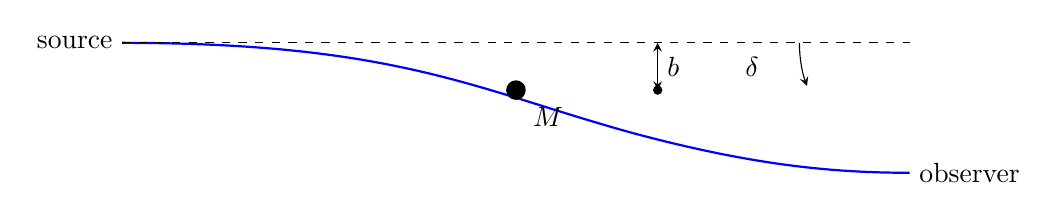
\begin{tikzpicture}[>=stealth, scale=1.0]
% asymptotes
\draw[thick,blue] (-5,0.6) .. controls (-1.5,0.6) and (-0.5,0.0) .. (1.5,-0.55) .. controls (3.0,-0.95) and (4.0,-1.05) .. (5,-1.05);
% straight reference path (undeflected)
\draw[dashed] (-5,0.6) -- (5,0.6);
% mass
\node[circle,fill=black,inner sep=2.5pt,label=below right:{$M$}] (M) at (0,0) {};
% impact parameter b: perpendicular distance from M to the dashed straight line
\draw[<->] (1.8,0) -- (1.8,0.6);
\node[right] at (1.8,0.30) {$b$};
% deflection angle delta between dashed and outgoing asymptote
\draw[->] (3.6,0.6) arc[start angle=180,end angle=200,radius=1.6];
\node at (3.0,0.30) {$\delta$};
% labels for source and observer ends
\node[left] at (-5,0.6) {source};
\node[right] at (5,-1.05) {observer};
% mark the closest approach point on the curve
\node[circle,fill,inner sep=1.2pt,label=above:{}] at (1.8,0.00) {};
\end{tikzpicture}
\end{center}

The dashed reference is the straight path the photon would have taken in the absence of the mass. The deflection angle $\delta$ is the angle between the incoming and outgoing asymptotes of the actual (curved) photon trajectory, measured against this straight line. The impact parameter $b$ is the perpendicular distance from $M$ to the undeflected reference line.

\subsection*{(b) Radial equation from the Lagrangian}

Schwarzschild line element ($B=1-2GM/(rc^2)$) in equatorial plane $\theta=\pi/2$:
\[ \de s^2=-c^2 B\,\de t^2+B^{-1}\de r^2+r^2\de\phi^2. \]
Lagrangian using affine parameter $\lambda$:
\[ 2\mathcal L=-c^2 B\,\dot t^2+B^{-1}\dot r^2+r^2\dot\phi^2,\qquad \dot{}\equiv \de/\de\lambda. \]
\textbf{Conserved quantities.} $t$ and $\phi$ are cyclic. Euler--Lagrange in $t$ gives $\de/\de\lambda(\partial\mathcal L/\partial\dot t)=0$:
\[ \frac{\de}{\de\lambda}\!\left(-c^2 B\,\dot t\right)=0\;\Rightarrow\;c^2 B\,\dot t=\text{const}\equiv\gamma_\infty c^2. \]
Euler--Lagrange in $\phi$ gives $\de/\de\lambda(\partial\mathcal L/\partial\dot\phi)=0$:
\[ \frac{\de}{\de\lambda}\!\left(r^2\dot\phi\right)=0\;\Rightarrow\;r^2\dot\phi=\text{const}\equiv\gamma_\infty J. \]
Collected:
\begin{equation}
c^2 B\,\dot t=\gamma_\infty c^2,\qquad r^2\dot\phi=\gamma_\infty J.
\label{eq:conserved}
\end{equation}
Here $\gamma_\infty c^2$ is the conserved energy per unit rest mass at infinity (so $\gamma_\infty\to1$ at rest, finite for a massive particle) and $J$ is the angular momentum per unit energy at infinity (units of length); equivalently $J/c$ is the impact-parameter combination for photons.

\textbf{Normalisation.} Carry the general particle relation $g_{\mu\nu}\dot x^\mu\dot x^\nu=-\epsilon c^2$ with $\epsilon=1$ (timelike) or $\epsilon=0$ (null):
\[ -c^2 B\dot t^2+B^{-1}\dot r^2+r^2\dot\phi^2=-\epsilon c^2. \]
Substitute $\dot t=\gamma_\infty/B$ from \eqref{eq:conserved}:
\[ -c^2 B\!\left(\frac{\gamma_\infty}{B}\right)^{\!2}+B^{-1}\dot r^2+r^2\dot\phi^2=-\epsilon c^2. \]
Simplify the first term:
\[ -\frac{c^2\gamma_\infty^2}{B}+B^{-1}\dot r^2+r^2\dot\phi^2=-\epsilon c^2. \]
Multiply through by $B$:
\[ -c^2\gamma_\infty^2+\dot r^2+B r^2\dot\phi^2=-\epsilon c^2 B. \]
Solve for $\dot r^2$:
\[ \dot r^2=c^2\gamma_\infty^2-\epsilon c^2 B-Br^2\dot\phi^2. \]
Divide by $\dot\phi^2$ to switch to $\phi$ as parameter:
\[ \left(\frac{\de r}{\de\phi}\right)^{\!2}=\frac{c^2\gamma_\infty^2}{\dot\phi^2}-\frac{\epsilon c^2 B}{\dot\phi^2}-Br^2. \]
Insert $1/\dot\phi^2=r^4/(\gamma_\infty J)^2$:
\[ \left(\frac{\de r}{\de\phi}\right)^{\!2}=\frac{c^2\gamma_\infty^2 r^4}{(\gamma_\infty J)^2}-\frac{\epsilon c^2 B r^4}{(\gamma_\infty J)^2}-Br^2. \]
Cancel $\gamma_\infty^2$ in the first term:
\[ \left(\frac{\de r}{\de\phi}\right)^{\!2}=\frac{c^2 r^4}{J^2}-Br^2-\frac{\epsilon c^2 B r^4}{\gamma_\infty^2 J^2}. \]
Factor $Br^2$ from the last two terms:
\[ \left(\frac{\de r}{\de\phi}\right)^{\!2}=\frac{c^2 r^4}{J^2}-Br^2\!\left(1+\frac{\epsilon c^2 r^2}{\gamma_\infty^2 J^2}\right). \]
Rearrange to the requested form:
\begin{equation}
\boxed{\;\left(\frac{\de r}{\de\phi}\right)^{\!2}+r^2 B\!\left(1+\frac{c^2 r^2}{\gamma_\infty^2 J^2}\right)=\frac{c^2 r^4}{J^2}.\;}
\label{eq:radial-eq}
\end{equation}
The displayed equation assumes the general (timelike) case $\epsilon=1$; for a photon $\epsilon=0$ and the $c^2 r^2/(\gamma_\infty^2 J^2)$ term drops, leaving $(\de r/\de\phi)^2+r^2 B=c^2 r^4/J^2$.

\textbf{Meaning of constants.} $\gamma_\infty$ is the Lorentz factor at infinity (energy per unit rest energy of the test particle), and $J=r^2\dot\phi/\gamma_\infty$ is the angular momentum per unit energy at infinity. The combination $J/c$ plays the role of impact parameter $b$ for the photon.

\subsection*{(c) Orbit equation $u''+u=(3GM/c^2)u^2$}

Take the photon limit ($\epsilon=0$) of \eqref{eq:radial-eq}:
\[ \left(\frac{\de r}{\de\phi}\right)^{\!2}+Br^2=\frac{c^2 r^4}{J^2}. \]
Identify the impact parameter $b=J/c$:
\[ \left(\frac{\de r}{\de\phi}\right)^{\!2}+Br^2=\frac{r^4}{b^2}. \]
Substitute $u=1/r$, so $r=1/u$ and $\de r/\de\phi=-u^{-2}\,\de u/\de\phi=-u'/u^2$:
\[ \left(\frac{\de r}{\de\phi}\right)^{\!2}=\frac{(u')^2}{u^4}. \]
Insert into the photon equation along with $r^2=1/u^2$, $r^4=1/u^4$:
\[ \frac{(u')^2}{u^4}+\frac{B}{u^2}=\frac{1}{u^4 b^2}. \]
Multiply through by $u^4$:
\[ (u')^2+u^2 B=\frac{1}{b^2}. \]
Expand $B=1-2GMu/c^2$:
\[ (u')^2+u^2-\frac{2GM u^3}{c^2}=\frac{1}{b^2}. \]
Differentiate w.r.t.\ $\phi$:
\[ 2u'u''+2u u'-\frac{6GM u^2 u'}{c^2}=0. \]
Divide by $2u'$ (non-degenerate):
\begin{equation}
\boxed{\;u''+u=\frac{3GM}{c^2}u^2.\;}
\label{eq:orbit}
\end{equation}

\textbf{Zeroth-order (no mass).} Set RHS$=0$:
\[ u_0''+u_0=0. \]
General solution:
\[ u_0=A\cos\phi+B\sin\phi. \]
Choose axes so the line of closest approach is at $\phi=\pi/2$ with $r=b$ (perpendicular distance $b$); this requires $u_0(\pi/2)=1/b$ and $u_0(0)=0$:
\[ u_0=\frac{\sin\phi}{b}. \]

\textbf{First-order.} Write $u=u_0+u_1$ with $u_1=O(1/c^2)$ and substitute into \eqref{eq:orbit}:
\[ (u_0''+u_0)+(u_1''+u_1)=\frac{3GM}{c^2}(u_0+u_1)^2. \]
The zeroth-order pair $u_0''+u_0=0$ cancels:
\[ u_1''+u_1=\frac{3GM}{c^2}(u_0+u_1)^2. \]
Expand the square and keep only $O(1/c^2)$ terms (drop $u_1^2$ and $u_0u_1$):
\[ u_1''+u_1=\frac{3GM}{c^2}u_0^2. \]
Insert $u_0=\sin\phi/b$:
\[ u_1''+u_1=\frac{3GM}{c^2}\,\frac{\sin^2\phi}{b^2}. \]
Apply $\sin^2\phi=(1-\cos 2\phi)/2$:
\begin{equation}
\boxed{\;u_1''+u_1=\frac{3GM}{c^2}\,\frac{1-\cos 2\phi}{2b^2}.\;}
\label{eq:u1-eq}
\end{equation}

\subsection*{(d) Einstein ring}

\textbf{Image.} The source, lens (black hole) and observer are colinear, so the deflection is rotationally symmetric about the line of sight. The photons reach the observer from every azimuth around the lens, producing a luminous ring on the sky --- an \emph{Einstein ring}.

\textbf{Geometry.} Let $\theta$ be the half-angle subtended at the observer between the lens and the ring image. The source lies on the optical axis at angular position $\beta=0$, and the photon is deflected by $\delta=4GM/(bc^2)$.

\begin{center}
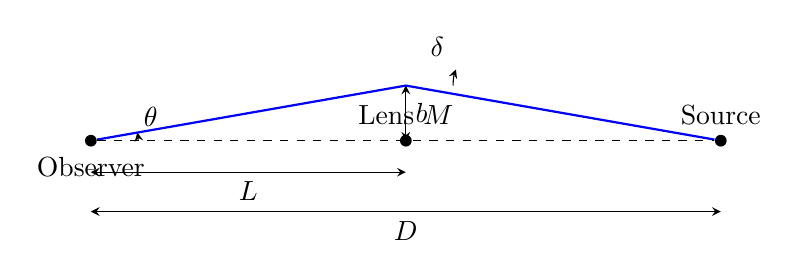
\begin{tikzpicture}[>=stealth,scale=1.0]
\node[circle,fill,inner sep=1.5pt,label=below:{Observer}] (O) at (0,0) {};
\node[circle,fill,inner sep=1.5pt,label=above:{Lens $M$}] (Lp) at (4,0) {};
\node[circle,fill,inner sep=1.5pt,label=above:{Source}] (S) at (8,0) {};
% photon path
\draw[blue,thick] (O) -- (4,0.7) -- (S);
\draw[dashed] (O) -- (S);
\draw[<->] (4,0) -- (4,0.7);
\node[right] at (4,0.35) {$b$};
\draw[->] (0.6,0) arc[start angle=0,end angle=10,radius=0.6];
\node[above right] at (0.55,0.05) {$\theta$};
\draw[->] (4.6,0.7) arc[start angle=180,end angle=160,radius=0.6];
\node[above] at (4.4,0.95) {$\delta$};
\draw[<->] (0,-0.4) -- (4,-0.4); \node[below] at (2,-0.4) {$L$};
\draw[<->] (0,-0.9) -- (8,-0.9); \node[below] at (4,-0.9) {$D$};
\end{tikzpicture}
\end{center}

Small-angle geometry at the lens plane sets the impact parameter:
\[ b=L\theta. \]
The undeflected ray from the observer at angle $\theta$ reaches the source plane at transverse offset $D\theta$; the deflection $\delta$ over distance $D-L$ subtracts $\delta(D-L)$; matching the on-axis source ($\beta=0$):
\[ D\theta-\delta(D-L)=0. \]
Rearrange:
\[ D\theta=\delta(D-L). \]
Insert $\delta=4GM/(bc^2)$ and $b=L\theta$:
\[ D\theta=\frac{4GM}{Lc^2\theta}(D-L). \]
Multiply by $\theta$:
\[ D\theta^2=\frac{4GM(D-L)}{Lc^2}. \]
Solve for $\theta^2$:
\[ \theta^2=\frac{4GM(D-L)}{c^2 LD}. \]
Take the square root and double for the angular diameter $2\theta$:
\begin{equation}
\boxed{\;2\theta=2\sqrt{\frac{4GM(D-L)}{c^2 LD}}.\;}
\label{eq:einstein-ring}
\end{equation}

%==============================================================
\section*{Question 4 --- Hubble flow and the Sachs--Wolfe effect}

\textbf{Problem.} Hubble recession of the Moon; whether to include $H_0$ in Earth--Moon dynamics; turnaround time of an over-dense sphere in EdS; analytic solution of the integral; Sachs--Wolfe $\Delta T/T$.

\subsection*{(a) Hubble recession of the Moon}

Hubble's law: $v=H_0 d$. Use $H_0\approx \SI{70}{km\,s^{-1}\,Mpc^{-1}}$, $1\,\text{Mpc}=\SI{3.086e19}{km}$:
\[ H_0=\frac{70}{3.086\times 10^{19}}\,\si{s^{-1}}=2.27\times 10^{-18}\,\si{s^{-1}}. \]
Distance $d=4\times 10^5\,\si{km}=4\times 10^{8}\,\si{m}$:
\[ v=H_0 d=(2.27\times 10^{-18})(4\times 10^{8})\,\si{m/s}. \]
Multiply:
\[ v=9.07\times 10^{-10}\,\si{m/s}. \]
Convert to cm per year: $1\,\text{yr}=3.156\times 10^{7}\,\si{s}$, $1\,\si{m}=100\,\si{cm}$:
\[ v=9.07\times 10^{-10}\times 3.156\times 10^{7}\times 100\,\si{cm/yr}. \]
Evaluate prefactor:
\[ 9.07\times 3.156\times 100=2862. \]
Powers of ten:
\[ 10^{-10}\times 10^{7}=10^{-3}. \]
Combine:
\[ \boxed{\;v_{\text{Hubble}}\approx 2.9\,\si{cm/yr}.\;} \]

\subsection*{(b) Should modellers include Hubble expansion?}

Measured recession $\SI{3.8}{cm/yr}$, comparable to the Hubble estimate $\sim\SI{2.9}{cm/yr}$, but the measured drift is dominated by tidal angular-momentum transfer, not cosmological expansion. \textbf{Decisive argument:} the Earth--Moon system is gravitationally bound and decoupled from the Hubble flow. A bound system does not partake in the cosmological expansion: the local geodesics tend to orbits in the (quasi-)Schwarzschild metric of the Earth, not to comoving cosmological geodesics. Quantitatively, the cosmological tidal acceleration on a bound orbit of size $r$ is
\[ a_{\text{cosmo}}\sim (\ddot a/a)\,r=-q H_0^2 r. \]
Evaluate $H_0^2$ first:
\[ H_0^2\simeq(2.3\times 10^{-18})^2\simeq 5.3\times 10^{-36}\,\si{s^{-2}}. \]
Multiply by $\tfrac12 r$ with $r=4\times 10^8\,\si{m}$, $q\sim 1/2$:
\[ |a_{\text{cosmo}}|\sim \tfrac12\cdot 5.3\times 10^{-36}\times 4\times 10^8\,\si{m\,s^{-2}}\sim 10^{-27}\,\si{m\,s^{-2}}. \]
Compare to the Newtonian Earth--Moon acceleration $GM_\oplus/r^2\sim 2.7\times 10^{-3}\,\si{m\,s^{-2}}$:
\[ a_{\text{cosmo}}/a_{\text{Newton}}\sim 10^{-25}. \]
\[ \boxed{\;\text{No: the Earth--Moon system is bound; cosmological expansion is negligible.}\;} \]

\subsection*{(c) Turnaround time integral}

\textbf{Setup.} Newtonian energy of a thin shell at $r$ enclosing total mass $M+\delta M$ (assume $\delta M$ a constant excess at all $r\le r_0$):
\[ \tfrac12\dot r^2-\frac{G(M+\delta M)}{r}=E. \]
\textbf{Initial condition.} At $r=r_0$, $\dot r$ equals the unperturbed EdS Hubble velocity. In EdS at critical density the energy of a comoving shell vanishes, giving:
\[ \tfrac12\dot r_0^2=\frac{GM}{r_0}. \]
Evaluate $E$ at $r=r_0$ using the perturbed energy expression:
\[ E=\tfrac12\dot r_0^2-\frac{G(M+\delta M)}{r_0}. \]
Substitute the EdS relation $\tfrac12\dot r_0^2=GM/r_0$:
\[ E=\frac{GM}{r_0}-\frac{G(M+\delta M)}{r_0}. \]
Combine fractions:
\[ E=-\frac{G\,\delta M}{r_0}. \]
\textbf{Equation of motion.} Substitute $E$ and rearrange the energy equation:
\[ \tfrac12\dot r^2=\frac{G(M+\delta M)}{r}-\frac{G\,\delta M}{r_0}. \]
Multiply by $2$:
\[ \dot r^2=\frac{2G(M+\delta M)}{r}-\frac{2G\,\delta M}{r_0}. \]
Define
\[ A=2G(M+\delta M),\qquad B=\frac{2G\,\delta M}{r_0}. \]
Rewrite:
\[ \dot r^2=\frac{A}{r}-B=\frac{A-Br}{r}. \]
\textbf{Turnaround.} $\dot r=0$ requires $r=A/B=(M+\delta M)r_0/\delta M$. Take the positive square root and separate variables:
\[ \de t=\sqrt{\frac{r}{A-Br}}\,\de r. \]
Integrate from $r_0$ to $A/B$:
\begin{equation}
\boxed{\;\int_{r_0}^{A/B}\!\sqrt{\frac{r}{A-Br}}\,\de r=\tau,\qquad A=2G(M+\delta M),\;B=\frac{2G\,\delta M}{r_0}.\;}
\label{eq:turnaround-int}
\end{equation}

\subsection*{(d) Approximate $\tau$}

Set lower limit to $0$ but keep $r_0$ in $A,B$. Substitute $u=Br/A$:
\[ r=\frac{A}{B}u,\qquad \de r=\frac{A}{B}\,\de u,\qquad A-Br=A(1-u). \]
Rewrite the integrand:
\[ \sqrt{\frac{r}{A-Br}}\,\de r=\sqrt{\frac{(A/B)u}{A(1-u)}}\cdot\frac{A}{B}\,\de u. \]
Simplify the radical:
\[ \sqrt{\frac{(A/B)u}{A(1-u)}}=\frac{1}{\sqrt{B}}\sqrt{\frac{u}{1-u}}. \]
Combine the prefactors:
\[ \tau\simeq\frac{A}{B^{3/2}}\int_0^1\!\sqrt{\frac{u}{1-u}}\,\de u. \]
Apply given integral $\int_0^1\!\sqrt{u/(1-u)}\,\de u=\pi/2$:
\[ \tau=\frac{\pi}{2}\,\frac{A}{B^{3/2}}. \]
Substitute $A=2G(M+\delta M)$ and $B=2G\,\delta M/r_0$:
\[ \tau=\frac{\pi}{2}\,\frac{2G(M+\delta M)}{\bigl[2G\,\delta M/r_0\bigr]^{3/2}}. \]
Move $r_0^{3/2}$ to the numerator:
\[ \tau=\frac{\pi}{2}\cdot\frac{2G(M+\delta M)\,r_0^{3/2}}{(2G\,\delta M)^{3/2}}. \]
Combine $2G$ powers using $2G/(2G)^{3/2}=(2G)^{-1/2}$:
\[ \tau=\frac{\pi}{2}\,\frac{(M+\delta M)\,r_0^{3/2}}{(2G)^{1/2}(\delta M)^{3/2}}. \]
For $\delta M\ll M$, drop $\delta M$ in the numerator:
\begin{equation}
\boxed{\;\tau\simeq\frac{\pi}{2}\sqrt{\frac{r_0^{3}}{2G\,\delta M}}\,\frac{M}{\delta M}=\frac{\pi M}{2\,\delta M}\sqrt{\frac{r_0^{3}}{2G\,\delta M}}.\;}
\label{eq:tau-final}
\end{equation}
Equivalently $\tau=(\pi/2)\,(M+\delta M)\,(r_0^3/(2G(\delta M)^3))^{1/2}$.

\subsection*{(e) Sachs--Wolfe $\Delta T/T$}

\textbf{Gravitational-potential term.} An over-density carries a Newtonian potential well of depth (with $\Phi=0$ at infinity):
\[ \Phi=-\frac{G\,\delta M}{r_0}. \]
The static weak-field metric gives the proper-time element at the well:
\[ \de\tau_{\text{local}}\simeq(1+\Phi/c^2)\,\de t. \]
With $\Phi<0$ the proper time at the well runs slower than the background coordinate time. A photon emitted from the well is gravitationally redshifted as it climbs out, lowering the observed temperature:
\[ \frac{\Delta T}{T}\bigg|_{\text{pot}}=\frac{\Phi}{c^2}. \]
Insert $\Phi=-G\,\delta M/r_0$:
\[ \frac{\Delta T}{T}\bigg|_{\text{pot}}=-\frac{G\,\delta M}{r_0 c^2}. \]

\textbf{Adiabatic-compression term.} The over-density alters the local scale factor by $\Delta R$ relative to the background. For radiation, the temperature scales inversely with the scale factor:
\[ T\propto \frac{1}{R}. \]
Differentiate logarithmically:
\[ \frac{\Delta T}{T}\bigg|_{\text{adiab}}=-\frac{\Delta R}{R}. \]

\textbf{Combine the two contributions.}
\begin{equation}
\boxed{\;\frac{\Delta T}{T}=-\frac{G\,\delta M}{r_0 c^2}-\frac{\Delta R}{R}.\;}
\label{eq:sachs-wolfe}
\end{equation}

\textbf{Sign of the second term.} For an over-density, the local region is more strongly self-gravitating, so its expansion is decelerated relative to the background, giving $\Delta R<0$. Hence $-\Delta R/R>0$: the compression \emph{raises} the local radiation temperature, partially compensating the (negative) potential-well term. The net Sachs--Wolfe result for adiabatic super-horizon perturbations is the well-known $\Delta T/T=\tfrac13\Phi/c^2$.

\end{document}
